% Created 2019-05-18 Sat 11:59
% Intended LaTeX compiler: pdflatex
\documentclass[12pt, a4paper]{article}
\usepackage[utf8]{inputenc}
\usepackage[T1]{fontenc}
\usepackage{graphicx}
\usepackage{grffile}
\usepackage{longtable}
\usepackage{wrapfig}
\usepackage{rotating}
\usepackage[normalem]{ulem}
\usepackage{amsmath}
\usepackage{textcomp}
\usepackage{amssymb}
\usepackage{capt-of}
\usepackage{hyperref}
\usepackage[style=authoryear,natbib]{biblatex}
\setlength\bibitemsep{\baselineskip}
\addbibresource{/Users/guilhermesalome/Dropbox/references.bib}
\usepackage[T1]{fontenc}
\usepackage{lmodern}
\usepackage{amsmath}
\usepackage{mathtools}
\usepackage{multirow}
\usepackage{booktabs}
\usepackage{bbm}
\usepackage[]{algorithm2e}
\newcommand\numberthis{\addtocounter{equation}{1}\tag{\theequation}}
\newcommand{\E}[1]{\mathbb{E}{\left[#1\right]}}
\newcommand{\EQ}[1]{\mathbb{E}_t^{\mathbb{Q}}{\left[#1\right]}}
\newcommand{\EP}[1]{\mathbb{E}_t^{\mathbb{P}}{\left[#1\right]}}
\newcommand{\e}[1]{\text{e}^{#1}}
\newcommand{\abs}[1]{\left\vert{#1}\right\vert}
\newcommand{\dis}{\overset{d}{\sim}}
\newcommand{\Var}[1]{\mathrm{Var}\left(#1\right)}
\newcommand{\Corr}[1]{\mathrm{Corr}\left(#1\right)}
\newcommand{\Normal}[1]{\mathcal{N}\left(0, #1\right)}
\newcommand{\Max}[1]{\text{max}\left\{#1\right\}}
\newcommand{\Set}[1]{\left\{#1\right\}}
\renewcommand{\ln}[1]{\text{ln}\left(#1\right)}
\DeclareMathOperator*{\argmin}{\arg\!\min}
\DeclareMathOperator*{\argmax}{\arg\!\max}
\DeclarePairedDelimiter\ceil{\lceil}{\rceil}
\DeclarePairedDelimiter\floor{\lfloor}{\rfloor}
\newcommand{\Poisson}[1]{\text{Poisson}\left(#1\right)}
\newcommand{\Uniform}[1]{\text{Unif}#1}
\newcommand{\Cov}[1]{\mathrm{Cov}\left(#1\right)}
\newtheorem{problem}{Problem}
\usepackage[hang,small,bf]{caption}
\usepackage[margin=1in]{geometry}
\usepackage{mathtools}
\usepackage{xcolor}
\usepackage{resizegather}
\usepackage{multirow}
\definecolor{darkgreen}{rgb}{0.1, 0.6, 0.1}
\usepackage{float}
\usepackage{fancyhdr}
\pagestyle{fancy}
\fancypagestyle{plain}{}
\fancyhf{}
\rfoot{Page \thepage}
\usepackage{ifthen}
\rhead{\ifthenelse{\value{page}=1}{Guilherme Salom\'{e}}{Summer \the\year}}
\lhead{\ifthenelse{\value{page}=1}{Econ890-01 Matlab}{Econ890-01 Matlab}}
\usepackage[numbered,framed]{matlab-prettifier}
\usepackage{listings}
\date{}
\title{Optimization}
\hypersetup{
 pdfauthor={Guilherme Salomé},
 pdftitle={Optimization},
 pdfkeywords={},
 pdfsubject={},
 pdfcreator={Emacs 26.1 (Org mode 9.2.1)},
 pdflang={English}}
\begin{document}

\maketitle
This lecture explores the optimization tools available in Matlab.
We begin with a light discussion on methods of minimization.
\section{The Optimization Problem}
\label{sec:org669c6c8}
Consider an optimization problem where we need to find the minimum value of a function \(f:\mathbb{R}\mapsto\mathbb{R}\) on some subset of its domain:
\begin{align*}
\min_{x\in D}{f(x)}
\end{align*}
We are interested in solving this problem.
However, it is not clear that a solution to this problem exists.
We know that if \(f\) is a \href{https://en.wikipedia.org/wiki/Continuous\_function}{continuous function} and \(D\) is a \href{https://en.wikipedia.org/wiki/Compact\_space}{compact set}, then by the \href{https://en.wikipedia.org/wiki/Extreme\_value\_theorem}{Weierstrass theorem} \(\exists x^*\in D:f(x^*)\leq f(x),\forall x\in D\).
Under these conditions, we know that a solution to the problem exists, but we still need a way to find it.
If the function \(f\) is not continuous, or \(D\) is not a compact set, then a solution may or may not exist.

Even though we cannot always guarantee that a solution exists, if a solution does exist, then it must satisfy a necessary condition.
If \(x_0\) is a point where \(f\) is minimized (or maximized) and \(f\) is differentiable at \(x_0\), then \(f'(x_0)=0\) (see \href{https://en.wikipedia.org/wiki/Fermat\%27s\_theorem\_(stationary\_points)}{Fermat's theorem on stationary points}).
This necessary condition motivates many of the optimization algorithms.

The algorithms for finding the argument that minimizes a function are divided in two types: direct search methods and gradient-based methods.
Direct search methods do not rely on the derivative of a function, and so can be applied to non differentiable functions.
These methods directly search for optimal points across the domain of a function.
An example of a direct search method is the \href{https://en.wikipedia.org/wiki/Golden-section\_search}{Golden-section search}.
Gradient-based methods use the derivative of a function to find a value \(x\) such that \(f'(x)=0\).
In these algorithms, the gradient can be explicitly computed or approximated numerically.
Examples of gradient-based algorithms are: \href{https://en.wikipedia.org/wiki/Bisection\_method}{Bisection method}, \href{https://en.wikipedia.org/wiki/Newton's\_method}{Newton-Raphson method} and \href{https://en.wikipedia.org/wiki/Secant\_method}{Secant method}.

These optimization methods apply to functions of a single variable.
However, they are building blocks for optimization methods for functions of many variables.
When it comes to optimization algorithms for functions of many variables, we can still divide the algorithms in the same two types.
Examples of direct search methods for multivariate functions are: \href{https://en.wikipedia.org/wiki/Powell's\_method}{Powell's method} and \href{https://en.wikipedia.org/wiki/Nelder–Mead\_method}{Nelder-Mead method}.
Some of the optimization methods that use the gradient are: \href{https://en.wikipedia.org/wiki/Newton's\_method}{Newton's method}, \href{https://en.wikipedia.org/wiki/Davidon–Fletcher–Powell\_formula}{DFP method}, \href{https://en.wikipedia.org/wiki/Broyden–Fletcher–Goldfarb–Shanno\_algorithm}{BFGS method} and the \href{https://en.wikipedia.org/wiki/Gradient\_descent}{Gradient Descent method}.

The methods above apply to unconstrained optimization problems.
However, in practice we usually have to deal with optimization problems that are subject to constraints:
\begin{equation*}
\begin{aligned}
& \underset{x\in\mathbb{R}^d}{\text{minimize}}
& & f(x)\\
& \text{subject to}
& & f_i(x) \leq b_i, i=1,\ldots, d
\end{aligned}
\end{equation*}
For constrained problems, some of the optimization methods are: \href{https://en.wikipedia.org/wiki/Penalty\_method}{Penalty function method}, \href{https://en.wikipedia.org/wiki/Augmented\_Lagrangian\_method}{Augmented Lagrangian method} and \href{https://en.wikipedia.org/wiki/Sequential\_quadratic\_programming}{Sequential quadratic programming}.
These methods either transform the constrained problem into an unconstrained problem with an added term that penalizes values that are outside the original constraints, or take extra care when looking through the domain to make sure the points satisfy the constrains.

Fortunately, we do not need to implement these algorithms, as most of them are already implemented in Matlab (and in various other programming languages).
A reference for all of the optimization algorithms mentioned above is \citet{A2015}, which also provides the code for these algorithms.
On the next sections we will discuss how to use the optimization methods available in Matlab, available via the \href{https://www.mathworks.com/help/optim/}{Optimization Toolbox} (should already be installed if you also installed the Econometrics Toolbox).
\section{Unconstrained Optimization (Gradient Based)}
\label{sec:org60723cd}
The function \href{https://www.mathworks.com/help/optim/ug/fminunc.html?s\_tid=doc\_ta}{\texttt{fminunc}} solves the optimization problem:
\begin{align*}
\min_{x}{f(x)}
\end{align*}
where \(f:\mathbb{R}^d\mapsto\mathbb{R}\) is a function of many variables that returns a scalar.
Remember that maximizing a function \(g\) is equivalent to minimizing \(-g\), so this solver can deal with minimization and maximization.

To use \texttt{fminunc} we need to supply it a function handle and an initial point.
It works with functions of a single variable:
\lstset{language=matlab,label= ,caption= ,captionpos=b,firstnumber=1,numbers=left,style=Matlab-editor}
\begin{lstlisting}
% polynomial example
f = @(x) x.^2;
x0 = 100;
[x, fx] = fminunc(f, x0);
% x: the argmin of the function
% fx: the value of the function at the minimizer
% the value of x is numerically close to zero (same for f'(x))
\end{lstlisting}

And also functions of many variables:
\lstset{language=matlab,label= ,caption= ,captionpos=b,firstnumber=1,numbers=left,style=Matlab-editor}
\begin{lstlisting}
% polynomial example on R2
f = @(x) 3*x(1).^2 + 2*x(1)*x(2) + x(2).^2 - 4*x(1) + 5*x(2);
% surface plot over a large region
x = linspace(-10000, 10000)';
y = linspace(-10000, 10000)';
[X, Y] = meshgrid(x, y);
Z = [X(:) Y(:)];
z = zeros(length(Z), 1);
for i = 1:length(Z)
    z(i) = f(Z(i, :));
end
z = reshape(z, length(y), length(x));
fig = surf(x, y, z);
hold on;
% find minimum
x0 = [1, 1];
[x, fx] = fminunc(f, x0);
% draw minimum on plot
scatter3(x(1), x(2), fx, 60, 'ro', 'filled');
\end{lstlisting}
We used \href{https://www.mathworks.com/help/matlab/ref/scatter3.html}{\texttt{scatter3}} to add a point at the minimum.
The surface plot is shown in Figure \ref{fig:org15a156f}.

\begin{figure}[H]
\centering
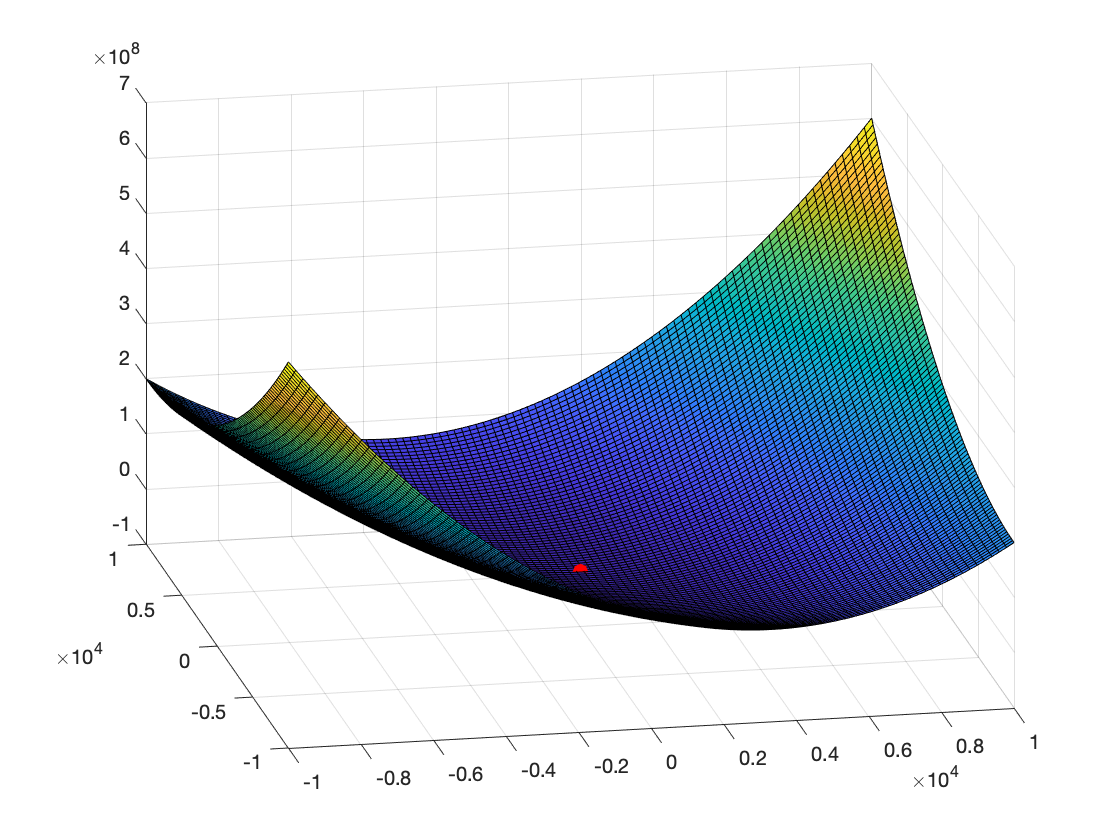
\includegraphics[width=8cm]{/Users/guilhermesalome/Teaching/Duke/Econ890 Matlab - 2019/supporting/matlab_minimizing_polynomial_surface.png}
\caption{\label{fig:org15a156f}
Surface of a Polynomial on \(\mathbb{R}^2\) and its Minimum.}
\end{figure}

Notice that in the examples above we did not supply the gradient of the function to \texttt{fminunc}.
In this case, Matlab is limited to numerically approximating the derivative, which can be unstable and is slow.
When no gradient is supplied, \texttt{fminunc} uses the \href{https://en.wikipedia.org/wiki/Quasi-Newton\_method}{Quasi-Newton method} and approximates the derivative with finite differences.
However, we can improve \texttt{fminunc} by also providing the gradient of the function.
In this case, \texttt{fminunc} can also use the \href{https://www.mathworks.com/help/optim/ug/unconstrained-nonlinear-optimization-algorithms.html}{Trust-Region method}.

To supply the gradient to \texttt{fminunc}, the function we want to minimize should output two values: the first is the objective function value (scalar), and the second is the gradient (vector) of the function.
\lstset{language=matlab,label= ,caption= ,captionpos=b,firstnumber=1,numbers=left,style=Matlab-editor}
\begin{lstlisting}
% rosenbrock.m
function [f, gradient] = rosenbrock(x)
% rosenbrock computes the Rosenbrock function
% reference: https://en.wikipedia.org/wiki/Rosenbrock_function
f = 100*(x(2)-x(1)^2)^2 + (1-x(1))^2;
gradient = [-400*(x(2)-x(1)^2)*x(1)-2*(1-x(1));
            200*(x(2)-x(1)^2)];

% check if user expects more than 1 output (i.e., also wants the gradient)
if nargout > 1
    gradient = [-400*(x(2)-x(1)^2)*x(1)-2*(1-x(1));
                200*(x(2)-x(1)^2)];
end
\end{lstlisting}
We use \href{https://www.mathworks.com/help/matlab/ref/nargout.html?s\_tid=doc\_ta}{\texttt{nargout}} to check how many outputs are expected.
\lstset{language=matlab,label= ,caption= ,captionpos=b,firstnumber=1,numbers=left,style=Matlab-editor}
\begin{lstlisting}
% in this case nargout is 1
f = rosenbrock([1; 0])
% in this case nargout is 2
[f, gradient] = rosenbrock([1; 0])
\end{lstlisting}

Let's visualize this function:
\lstset{language=matlab,label= ,caption= ,captionpos=b,firstnumber=1,numbers=left,style=Matlab-editor}
\begin{lstlisting}
x = linspace(-2, 2);
y = linspace(-3, 3);
[X, Y] = meshgrid(x, y);
Z = [X(:) Y(:)];
z = zeros(length(Z), 1);
for i = 1:length(Z)
    z(i) = rosenbrock(Z(i, :));
end
z = reshape(z, length(y), length(x));
fig = surf(x, y, z);
hold on;
% actual minimum
scatter3(1, 1, 0, 60, 'ro', 'filled');
\end{lstlisting}
The graph of the function is shown in Figure \ref{fig:orgc91c718}.

\begin{figure}[H]
\centering
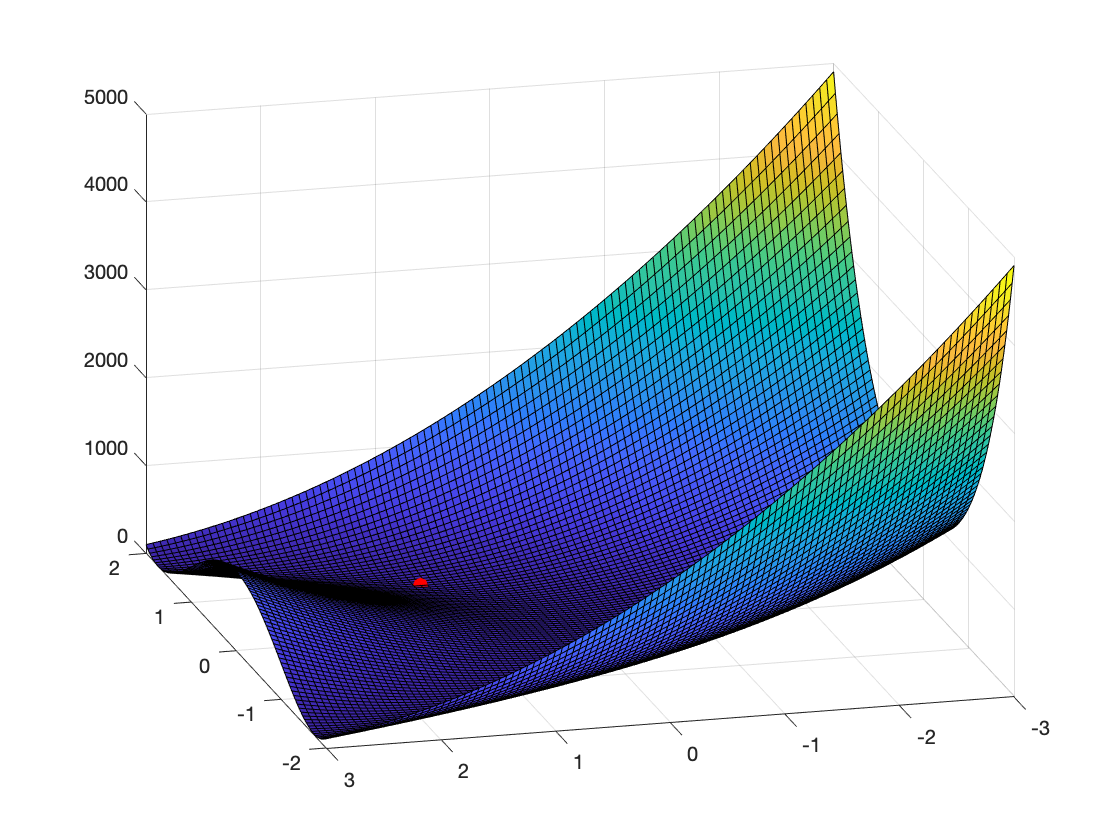
\includegraphics[width=8cm]{/Users/guilhermesalome/Teaching/Duke/Econ890 Matlab - 2019/supporting/matlab_rosenbrock_surface.png}
\caption{\label{fig:orgc91c718}
Rosenbrock Function and Global Minimum.}
\end{figure}

We can now call \texttt{fminunc} and pass it an \texttt{options} argument, which specifies that the gradient of the function is also available.
The \texttt{options} argument is created with the function \href{https://www.mathworks.com/help/optim/ug/optimoptions.html?s\_tid=doc\_ta}{\texttt{optimoptions}}.
\lstset{language=matlab,label= ,caption= ,captionpos=b,firstnumber=1,numbers=left,style=Matlab-editor}
\begin{lstlisting}
% set up options for fminunc
% The first argument is the optimizer we are using, in this case,
% 'fminunc'. The other arguments are name-value pairs.
options = optimoptions('fminunc', ...
                       'SpecifyObjectiveGradient', true, ...
                       'Algorithm', 'trust-region');
[x, fx] = fminunc(@rosenbrock, [-1, 2], options);
\end{lstlisting}

We can also use the \texttt{options} argument to display the algorithm iterations as they occur:
\lstset{language=matlab,label= ,caption= ,captionpos=b,firstnumber=1,numbers=left,style=Matlab-editor}
\begin{lstlisting}
options = optimoptions('fminunc', ...
                       'SpecifyObjectiveGradient', true, ...
                       'Algorithm', 'trust-region', ...
                       'Display', 'iter');
[x, fx, exitflag, output] = fminunc(@rosenbrock, [-1, 2], options);
\end{lstlisting}
The \texttt{output} is a \texttt{struct} containing information about the optimization, and the \texttt{exitflag} indicates a number representing the type of solution obtained (1 for local minima, see \href{https://www.mathworks.com/help/optim/ug/fminunc.html?s\_tid=doc\_ta\#butpb7p-exitflag}{\texttt{exitflag}} for the meaning of the other values).

During the optimization process, \texttt{fminunc} computes the gradient and the Hessian of the function.
We can obtain the gradient and the Hessian at the end of the minimization process:
\lstset{language=matlab,label= ,caption= ,captionpos=b,firstnumber=1,numbers=left,style=Matlab-editor}
\begin{lstlisting}
[x, fx, exitflag, output, grad, hess] = fminunc(@rosenbrock, [-1, 2], options);
\end{lstlisting}

There are other options that we can set:
\begin{itemize}
\item \texttt{MaxIterations}: maximum number of iterations (default is 400);
\item \texttt{OptimalityTolerance}: tolerance for \(f'(x)=0\) (default is \(10^{-6}\))
\item \texttt{StepTolerance}: tolerance for the step size (default is \(10^{-6}\))
\item \texttt{PlotFcn}: plot the function value as it is optimized
\item \texttt{UseParallel}: approximates the gradient in parallel
\end{itemize}

For example, with \texttt{PlotFcn} we can see the evolution of the optimization graphically:
\lstset{language=matlab,label= ,caption= ,captionpos=b,firstnumber=1,numbers=left,style=Matlab-editor}
\begin{lstlisting}
plots = ["optimplotx", "optimplotfval", ...
         "optimplotstepsize", "optimplotfirstorderopt"];
options = optimoptions('fminunc', ...
                       'SpecifyObjectiveGradient', true, ...
                       'Algorithm', 'trust-region', ...
                       'Display', 'iter', ...
                       'PlotFcn', plots);
[x, fx, exitflag, output] = fminunc(@rosenbrock, [-1, 2], options);
\end{lstlisting}
See Figure \ref{fig:org35a268a}.

\begin{figure}[H]
\centering
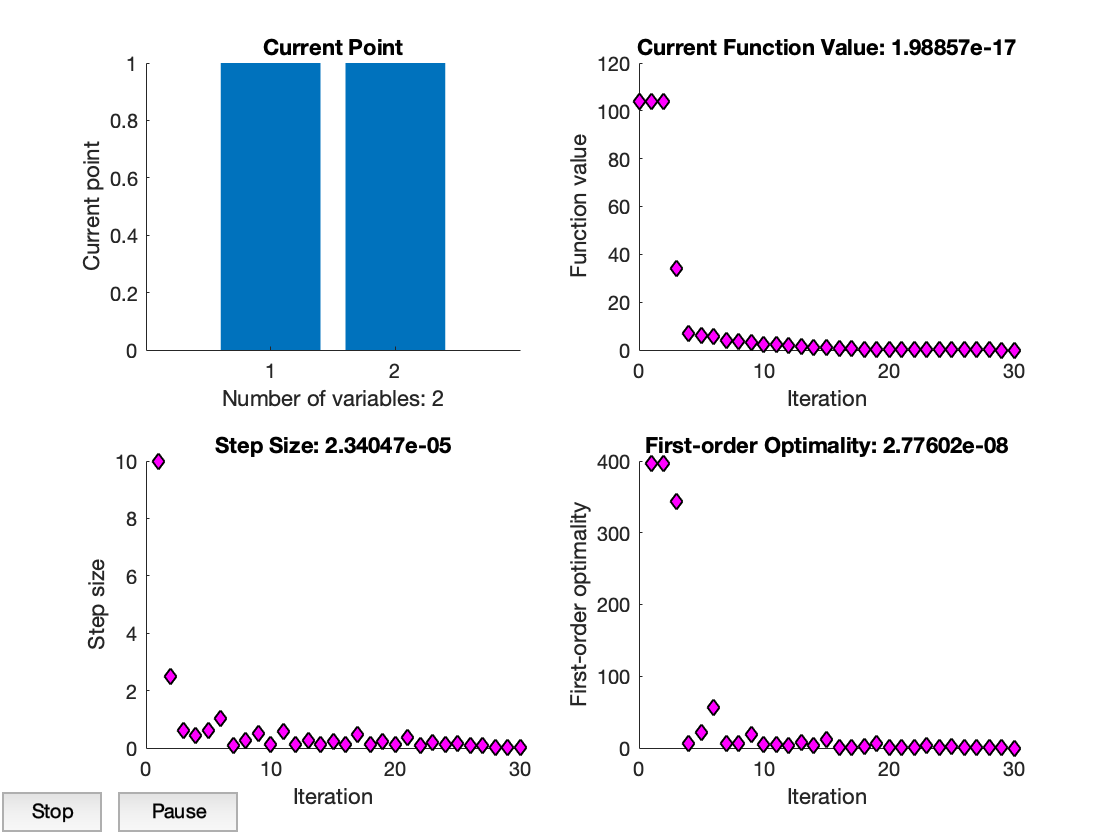
\includegraphics[width=8cm]{/Users/guilhermesalome/Teaching/Duke/Econ890 Matlab - 2019/supporting/matlab_optimization_evolution.png}
\caption{\label{fig:org35a268a}
Function Value and Inputs During Minimization.}
\end{figure}

A complete list of options is available at the \href{https://www.mathworks.com/help/optim/ug/fminunc.html?s\_tid=doc\_ta\#butpb7p-options}{\texttt{fminunc} reference page}.
\section{Unconstrained Optimization (Direct Search)}
\label{sec:org3a874fd}
The function \href{https://www.mathworks.com/help/matlab/ref/fminsearch.html?s\_tid=doc\_ta}{\texttt{fminsearch}} also solves an unconstrained minimization problem, but uses a direct search method that does not rely on the gradient of the function being minimized.
Specifically, \texttt{fminsearch} uses the \href{https://www.mathworks.com/help/optim/ug/fminsearch-algorithm.html}{Nelder-Mead algorithm}.

The usage of \texttt{fminsearch} is similar to \texttt{fminunc}:
\lstset{language=matlab,label= ,caption= ,captionpos=b,firstnumber=1,numbers=left,style=Matlab-editor}
\begin{lstlisting}
[x, fx] = fminsearch(@rosenbrock, [-1, 2]);
\end{lstlisting}

To specify extra options, however, we use the function \href{https://www.mathworks.com/help/matlab/ref/optimset.html}{\texttt{optimset}} (it is different from the one used with \texttt{fminunc}):
\lstset{language=matlab,label= ,caption= ,captionpos=b,firstnumber=1,numbers=left,style=Matlab-editor}
\begin{lstlisting}
options = optimset('Display', 'iter');
[x, fx, exitflag, output] = fminsearch(@rosenbrock, [-1, 2], options);
\end{lstlisting}
Notice that \texttt{fminsearch} does not return the gradient and hessian of the function at the minimizer, since it does not use derivatives.
\section{Constrained Optimization}
\label{sec:org5bcde58}
The function \href{https://www.mathworks.com/help/optim/ug/fmincon.html?s\_tid=doc\_ta}{\texttt{fmincon}} solves the following constrained minimization problem:
\begin{equation*}
\begin{aligned}
& \underset{x\in\mathbb{R}^d}{\text{minimize}} & & f(x)\\
& \text{subject to} & & \begin{cases}
c(x) \leq 0\\
{ceq}(x) = 0\\
A\cdot x\leq b\\
{Aeq}\cdot x = {beq}\\
lb \leq x \leq ub
\end{cases}
\end{aligned}
\end{equation*}
Where: \(f:\mathbb{R}^d\mapsto\mathbb{R}\), \(c:\mathbb{R}^d\mapsto\mathbb{R}^{k_1}\), \({ceq}:\mathbb{R}^d\mapsto\mathbb{R}^{k_2}\), \(A\in\mathbb{R}^{k_3\times d}\) and \(b\in\mathbb{R}^{k_3\times 1}\), \({Aeq}\in\mathbb{R}^{k_4\times d}\) and \({beq}\in\mathbb{R}^{k_4\times 1}\), and \(x\), \(lb\) and \(ub\) are vectors of length \(d\).

We can call \texttt{fmincon} using several different configurations, which we explore in the next subsections.
\subsection{Linear Inequality Constraint}
\label{sec:org45daa11}
Let's minimize Rosenbrock's function with the constraint that \(x_1 + 2x_2 \leq 1\):
\lstset{language=matlab,label= ,caption= ,captionpos=b,firstnumber=1,numbers=left,style=Matlab-editor}
\begin{lstlisting}
%% Let's minimize Rosenbrock's function with an additional
% constraint
A = [1 2];
x0 = [-1; 2];
b = 1;
%% Visualize the graph of the function and the linear constraint
x = linspace(-2, 2, 60);
y = linspace(-3, 3, 60);
[X, Y] = meshgrid(x, y);
Z = [X(:) Y(:)];
z = zeros(length(Z), 1);
for i = 1:length(Z)
    z(i) = rosenbrock(Z(i, :));
end
z = reshape(z, length(y), length(x));
fig = surf(x, y, z);
fig.FaceAlpha = 0.8;
colormap cool;
hold on;
% add constraint
X1 = [2;2;-2;-2];
X2 = [-3;-0.5;3/2;-3];
fill(X1, X2, 'green');
% actual minimum
scatter3(1, 1, 0, 60, 'ro', 'filled');
%% Minimize the function under the constraint
[x, fx] = fmincon(@rosenbrock, x0, A, b);
%% Add minimization result to figure
scatter3(x(1), x(2), fx, 60, 'ko', 'filled');
% add labels and legend
xlabel('x_1');
ylabel('x_2');
legend(["Rosenbrock's Function", "Linear Constraint", ...
        "Global Minimum", "Constrained Minimum"], ...
       "Location", "northwest");
\end{lstlisting}
We can visualize the result of the constrained minimization in Figure \ref{fig:org788df26} below.

\begin{figure}[H]
\centering
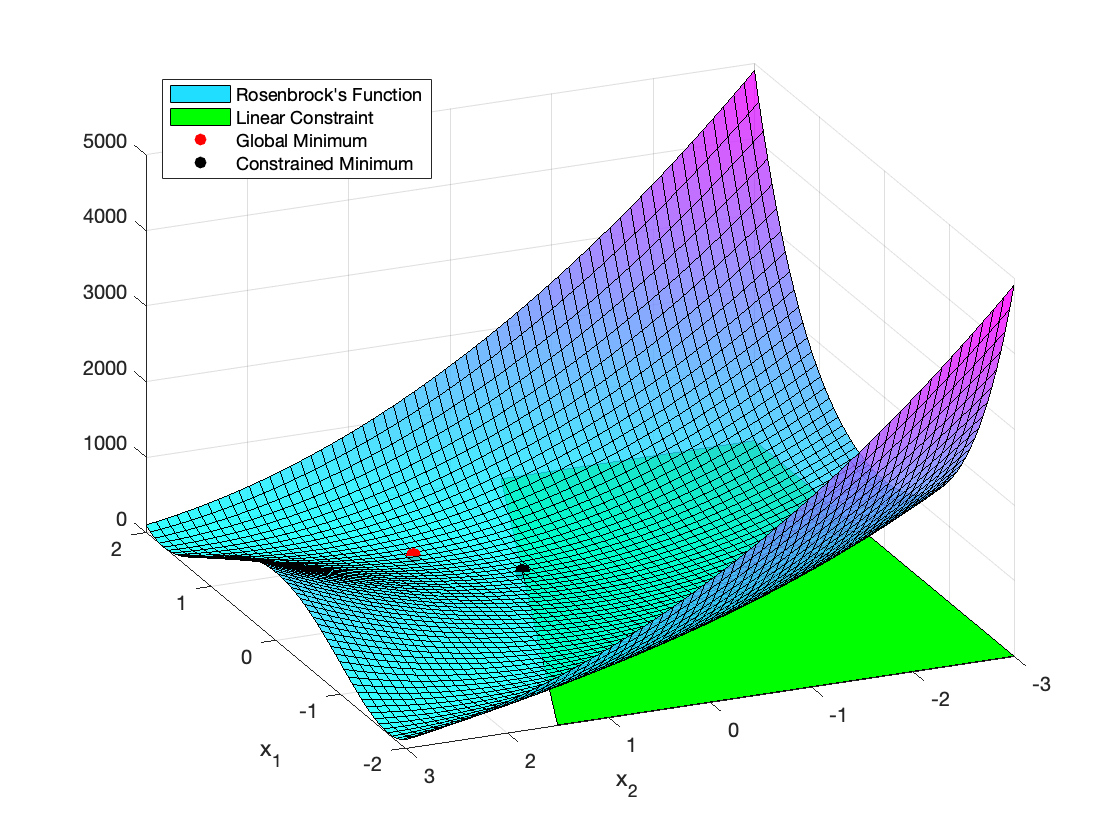
\includegraphics[width=8cm]{/Users/guilhermesalome/Teaching/Duke/Econ890 Matlab - 2019/supporting/matlab_minimization_constrained.png}
\caption{\label{fig:org788df26}
Minimization of the Rosenbrock's Function under a Linear Constraint.}
\end{figure}
\subsection{Linear Inequality and Equality Constraints}
\label{sec:orgc88d1df}
Let's add a linear equality constraint:
\lstset{language=matlab,label= ,caption= ,captionpos=b,firstnumber=1,numbers=left,style=Matlab-editor}
\begin{lstlisting}
%% Let's minimize Rosenbrock's function with two linear constraints
% inequality constraint: x(1) + 2*x(1) <= 1
A = [1 2];
b = 1;
% equality constraint: 2*x(1) + x(2) = 1
Aeq = [2 1];
beq = 1;
%% Visualize function and constraints
x = linspace(-2, 2, 60);                % x1
y = linspace(-3, 3, 60);                % x2
[X, Y] = meshgrid(x, y);
Z = [X(:) Y(:)];
z = zeros(length(Z), 1);
for i = 1:length(Z)
    z(i) = rosenbrock(Z(i, :));
end
z = reshape(z, length(y), length(x));
fig = surf(x, y, z);
fig.FaceAlpha = 0.8;
colormap cool;
hold on;
% add inequality constraint
X1 = [2;2;-2;-2];
X2 = [-3;-0.5;3/2;-3];
fill(X1, X2, 'green');
% add equality constraint
plot(x, 1- 2.*x, 'k', 'LineWidth', 2);
% actual minimum
scatter3(1, 1, 0, 60, 'ro', 'filled');
%% Minimize the function under the constraint
x0 = [0; 0.5];
[x, fx] = fmincon(@rosenbrock, x0, A, b, Aeq, beq);
%% Add minimization result to figure
scatter3(x(1), x(2), fx, 60, 'ko', 'filled');
% add labels and legend
xlim([-2, 2]);
ylim([-3, 3]);
xlabel('x_1');
ylabel('x_2');
legend(["Rosenbrock's Function", "Inequality Constraint", ...
        "Equality Constraint", "Global Minimum", ...
        "Constrained Minimum"], "Location", "northwest");

\end{lstlisting}

We can visualize the result of the constrained minimization in Figure \ref{fig:org968d02a} below.
\begin{figure}[H]
\centering
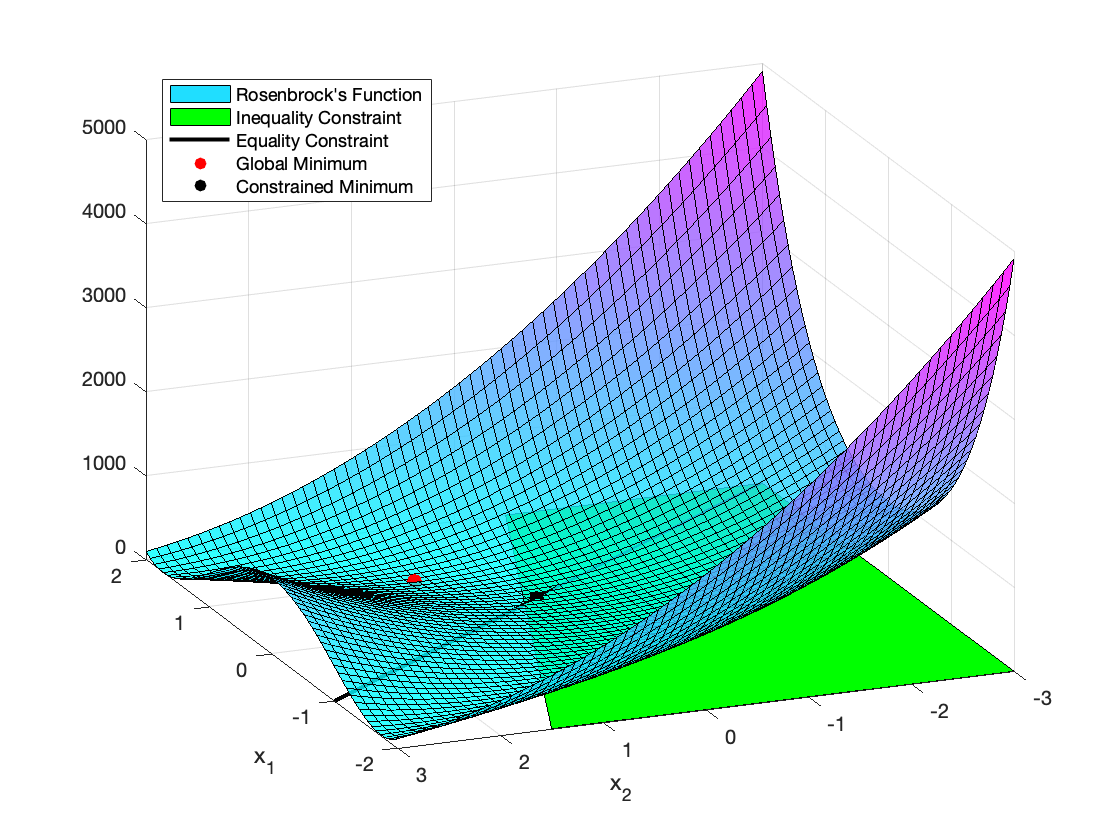
\includegraphics[width=8cm]{/Users/guilhermesalome/Teaching/Duke/Econ890 Matlab - 2019/supporting/matlab_minimization_two_linear_constraints.png}
\caption{\label{fig:org968d02a}
Minimization of the Rosenbrock's Function under a Linear Inequality Constraint and a Linear Equality Constraint.}
\end{figure}

\subsection{Linear Equality Constraint}
\label{sec:org3f62cad}
If we did not want to specify the linear inequality constraint, then we can pass an empty matrix \texttt{[]} as the inputs for \texttt{A} and \texttt{b}:
\lstset{language=matlab,label= ,caption= ,captionpos=b,firstnumber=1,numbers=left,style=Matlab-editor}
\begin{lstlisting}
%% Let's minimize Rosenbrock's function with a linear equality constraint
% equality constraint: 2*x(1) + x(2) = 1
Aeq = [2 1];
beq = 1;
%% Visualize function and constraints
x = linspace(-2, 2, 60);                % x1
y = linspace(-3, 3, 60);                % x2
[X, Y] = meshgrid(x, y);
Z = [X(:) Y(:)];
z = zeros(length(Z), 1);
for i = 1:length(Z)
    z(i) = rosenbrock(Z(i, :));
end
z = reshape(z, length(y), length(x));
fig = surf(x, y, z);
fig.FaceAlpha = 0.8;
colormap cool;
hold on;
% add equality constraint
plot(x, 1- 2.*x, 'k', 'LineWidth', 2);
% actual minimum
scatter3(1, 1, 0, 60, 'ro', 'filled');
%% Minimize the function under the constraint
x0 = [0.5; 0];
[x, fx] = fmincon(@rosenbrock, x0, [], [], Aeq, beq);
%% Add minimization result to figure
scatter3(x(1), x(2), fx, 60, 'ko', 'filled');
% add labels and legend
xlim([-2, 2]);
ylim([-3, 3]);
xlabel('x_1');
ylabel('x_2');
legend(["Rosenbrock's Function", "Equality Constraint", "Global Minimum", ...
        "Constrained Minimum"], "Location", "northwest");
\end{lstlisting}

We can visualize the result of the constrained minimization in Figure \ref{fig:orgf116d16} below.
\begin{figure}[H]
\centering
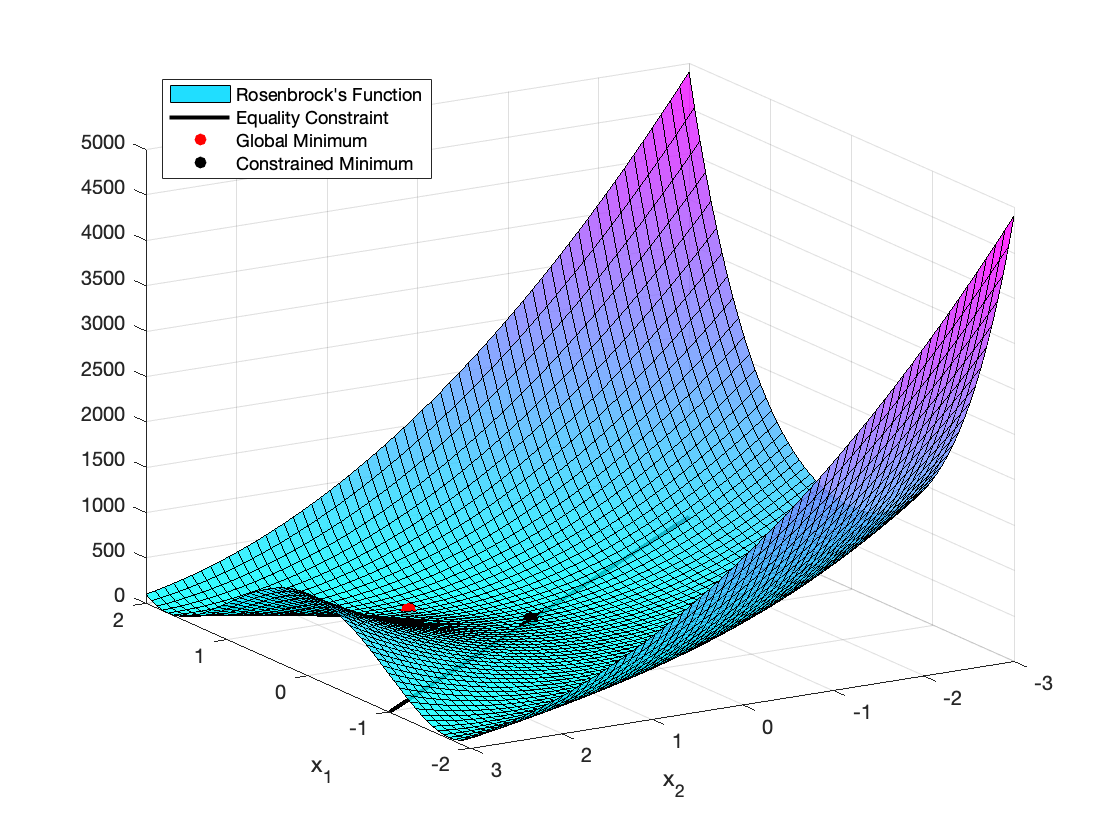
\includegraphics[width=8cm]{/Users/guilhermesalome/Teaching/Duke/Econ890 Matlab - 2019/supporting/matlab_minimization_only_equality_constraint.png}
\caption{\label{fig:orgf116d16}
Minimization of the Rosenbrock's Function under a Linear Equality Constraint.}
\end{figure}
\subsection{Bound Constraints}
\label{sec:orgc11850b}
We now consider bound constraints: \({lb}\leq x\leq {ub}\).
\lstset{language=matlab,label= ,caption= ,captionpos=b,firstnumber=1,numbers=left,style=Matlab-editor}
\begin{lstlisting}
%% Specify a function
f = @(x) (1+x(1)/(1+x(2)) - 3*x(1)*x(2) + x(2)*(1+x(1)));
%% Visualize f
x = linspace(-0.5, 1.5, 60);                % x1
y = linspace(-0.5, 3, 60);                % x2
[X, Y] = meshgrid(x, y);
Z = [X(:) Y(:)];
z = zeros(length(Z), 1);
for i = 1:length(Z)
    z(i) = f(Z(i, :));
end
z = reshape(z, length(y), length(x));
fig = surf(x, y, z);
hold on;
xlabel('x1');
ylabel('x2');
%% Define bound constraint
% positive values of x
lb = [0; 0];
ub = [1; 2];
%% Minimize function
x0 = [0.5, 1];
[x, fx] = fmincon(f, x0, [], [], [], [], lb, ub);
%% Visualize minima
scatter3(x0(1), x0(2), f(x0), 60, 'ko', 'filled');
scatter3(x(1), x(2), fx, 60, 'ro', 'filled');
%% Minimize function
x0 = x0./5;
[x, fx] = fmincon(f, x0, [], [], [], [], lb, ub);
%% Visualize minima
scatter3(x0(1), x0(2), f(x0), 60, 'ko', 'filled');
scatter3(x(1), x(2), fx, 60, 'ro', 'filled');
legend(["Graph of f", "Initial Guess", "Local Minimum", ...
        "Another Initial Guess", "Another Local Minimum"], ...
       "Location", "northwest");
\end{lstlisting}

Figure \ref{fig:orgf804ef8} below displays the function and the local minima we found in the constrained region.
\begin{figure}[H]
\centering
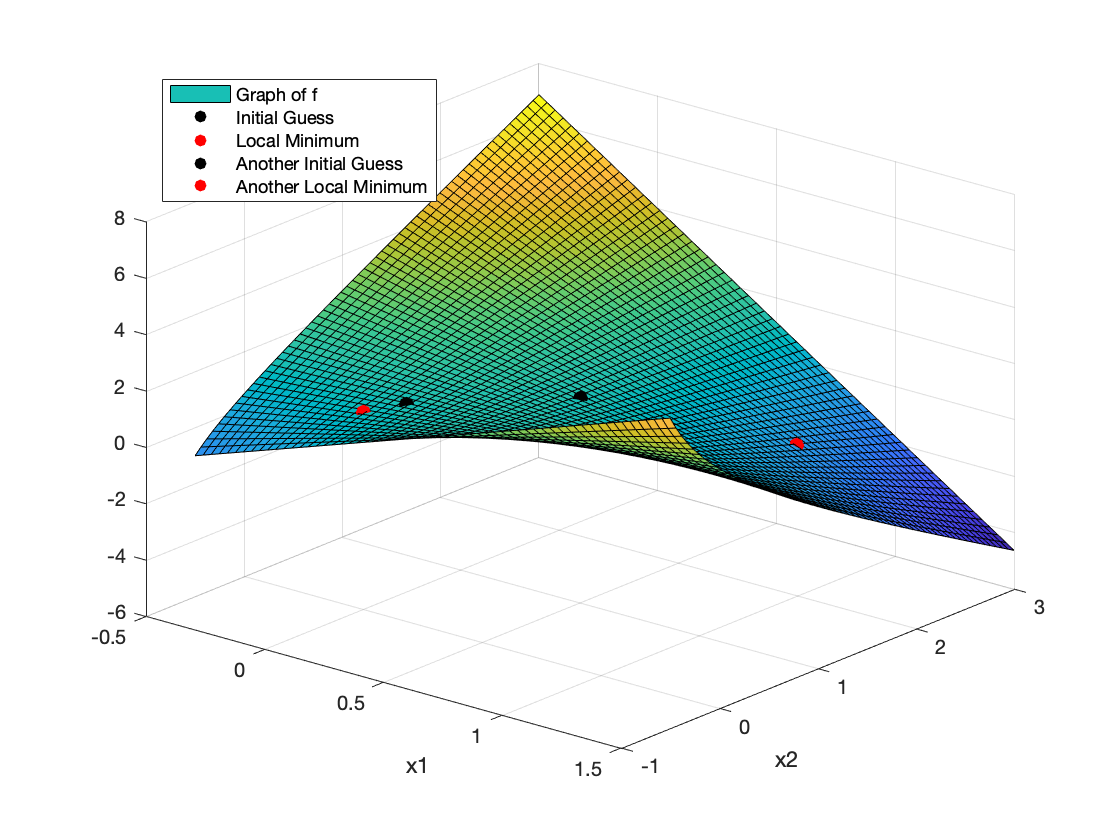
\includegraphics[width=8cm]{/Users/guilhermesalome/Teaching/Duke/Econ890 Matlab - 2019/supporting/matlab_minimization_bound_constraint.png}
\caption{\label{fig:orgf804ef8}
Minimization of a Function Under Bound Constraints.}
\end{figure}
We can find the global minima in this region by comparing the objective function value at the two local minima.
\subsection{Nonlinear Constraint}
\label{sec:orga1a2222}
Let's find the minimum of the Rosenbrock's function when the domain is constrained to a circle.
First, we specify the nonlinear constraint by creating a new function.
This function must take an input \(x\), and must have two outputs: \(c(x)\) and \({ceq}(x)\).
If the nonlinear inequality constraint or the nonlinear equality constraint are not used, then the function should simply output \texttt{[]}.

Remember that a point \((x,y)\) is in a circle centered at \((a,b)\) with radius \(r\) if:
\begin{align*}
\left\Vert (x,y) - (a,b) \right\Vert \leq r
\end{align*}
Now, \texttt{fmincon} considers the nonlinear constraint to be of the form \(c(x)\leq 0\).
So we need to convert the inequality above to be of that form.
We can also write the inequality in terms of squares instead of square-root, since computing the square of a number is faster than computing its square-root:
\begin{align*}
\left\Vert (x,y) - (a,b) \right\Vert \leq r
&\iff (x-a)^2 + (y-b)^2 \leq r^2\\
&\iff (x-a)^2 + (y-b)^2 - r^2 \leq 0
\end{align*}
We can now write this inequality in a function:
\lstset{language=matlab,label= ,caption= ,captionpos=b,firstnumber=1,numbers=left,style=Matlab-editor}
\begin{lstlisting}
% in_circle.m
function [c, ceq] = in_circle(point, center, radius)
% in_cirlce returns a negative number if the point is in the circle,
% otherwise returns a positive number
c = sum((point - center).^2) - radius^2; % <= 0
ceq = [];                                % == 0
\end{lstlisting}

Now, we can minimize Rosenbrock's function subject to this nonlinear constraint:
\lstset{language=matlab,label= ,caption= ,captionpos=b,firstnumber=1,numbers=left,style=Matlab-editor}
\begin{lstlisting}
%% Minimize function
fun = @(x) (in_circle(x, [0.5 0.5], 0.5));
x0 = [0.5 1];
[x_min, f_min] = fmincon(fun, x0, [], [], [], [], [], [], fun);
%% Visualize problem
x = linspace(-0.5, 1.5, 60);                % x1
y = linspace(-0.5, 1.5, 60);                % x2
[X, Y] = meshgrid(x, y);
Z = [X(:) Y(:)];
z = zeros(length(Z), 1);
for i = 1:length(Z)
    z(i) = rosenbrock(Z(i, :));
end
z = reshape(z, length(y), length(x));
fig = surf(x, y, z);
fig.FaceAlpha = 0.6;
colormap cool;
hold on;
r = rectangle('Position', [0 0 1 1], 'Curvature', [1 1], ...
              'FaceColor', 'white');
scatter3(x0(1), x0(2), rosenbrock(x0), 120, 'ko', 'filled');
scatter3(x_min(1), x_min(2), f_min, 120, 'ro', 'filled');
xlabel('x1');
ylabel('x2');
xlim([-0.5 1.5]);
ylim([-0.5 1.5]);
legend(["Rosenbrock's Function", "Initial Guess", "Local Minimum"], ...
       'location', 'northwest');
\end{lstlisting}
We used the function \href{https://www.mathworks.com/help/matlab/ref/rectangle.html}{\texttt{rectangle}} to draw the circle.
The optimization result is shown in Figure \ref{fig:org0871b36}.

\begin{figure}[H]
\centering
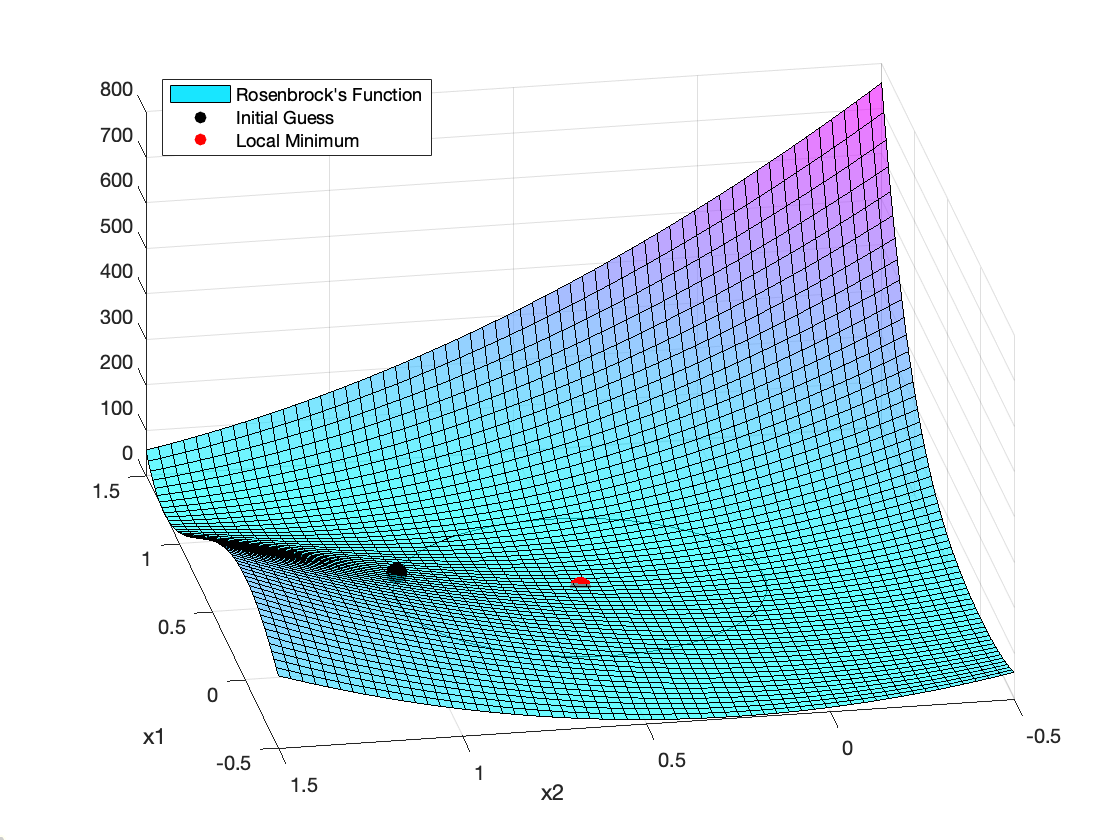
\includegraphics[width=8cm]{/Users/guilhermesalome/Teaching/Duke/Econ890 Matlab - 2019/supporting/matlab_nonlinear_constraint_circle.png}
\caption{\label{fig:org0871b36}
Minimization of Rosenbrock's Function Under a Nonlinear Constraint.}
\end{figure}
\subsection{Options and Algorithms}
\label{sec:org6a7ecc3}
There are five algorithm options for \texttt{fmincon}: \href{https://www.mathworks.com/help/optim/ug/constrained-nonlinear-optimization-algorithms.html\#brnpd5f}{\texttt{interior-point}} (default), \href{https://www.mathworks.com/help/optim/ug/constrained-nonlinear-optimization-algorithms.html\#brnpeek}{\texttt{trust-region-reflective}}, \href{https://www.mathworks.com/help/optim/ug/constrained-nonlinear-optimization-algorithms.html\#bsgppl4}{\texttt{sqp}}, \texttt{sqp-legacy} and \href{https://www.mathworks.com/help/optim/ug/constrained-nonlinear-optimization-algorithms.html\#brnox01}{\texttt{active-set}}.
The links above lead to the descriptions of each algorithm.
The general reasoning for each of the algorithms is the following:
\begin{itemize}
\item Interior Point: Large-scale algorithm (uses sparse matrices, less memory). Constraints are satisfied at all times.
\item Trust Region Reflective: Large-scale algorithm (uses sparse matrices, less memory). Requires the gradient of the function. Can only have bound constraints or linear equality constraints, but not both.
\item SQP: Medium-scale algorithm (uses dense matrices, uses more memory, more accurate). Constraints are satisfied at all times. The legacy version is slower and uses more memory.
\item Active Set: Medium-scale algorithm (uses dense matrices, uses more memory, more accurate). Is able to take large steps. Can deal with non-smooth constraints.
\end{itemize}

We can choose the algorithm by setting options for \texttt{fmincon} using \href{https://www.mathworks.com/help/optim/ug/optimoptions.html?s\_tid=doc\_ta}{\texttt{optimoptions}}.
\lstset{language=matlab,label= ,caption= ,captionpos=b,firstnumber=1,numbers=left,style=Matlab-editor}
\begin{lstlisting}
% Minimize Rosenbrock's on a unit circle
unit_circle = @(x) (in_circle(x, [0; 0], 1));
x0 = [0,0];
% Set options to display minimization progression
options = optimoptions('fmincon', 'Display', 'iter');

% Minimize with the default algorithm
options.Algorithm = 'interior-point';
[x_min, f_min] = fmincon(@rosenbrock,x0,[],[],[],[],[],[],unit_circle,options)

% Minimize with the sqp algorithm
options.Algorithm = 'sqp';
[x_min, f_min] = fmincon(@rosenbrock,x0,[],[],[],[],[],[],unit_circle,options)

% Minimize with the active-set algorithm
options.Algorithm = 'active-set';
[x_min, f_min] = fmincon(@rosenbrock,x0,[],[],[],[],[],[],unit_circle,options)

% Minimize with the trust-region-reflective algorithm
% will not work due to constraints (and gradient)
options.Algorithm = 'trust-region-reflective';
[x_min, f_min] = fmincon(@rosenbrock,x0,[],[],[],[],[],[],unit_circle,options)
\end{lstlisting}
\subsection{Including the Gradient}
\label{sec:org1825faa}
To include the gradient we specify the objective function to return two outputs.
The first is the value of the function, and the second is the gradient of the function.
We can then specify the option \texttt{SpecifyObjectiveGradient} to be \texttt{true}:
\lstset{language=matlab,label= ,caption= ,captionpos=b,firstnumber=1,numbers=left,style=Matlab-editor}
\begin{lstlisting}
% Minimize Rosenbrock's function over positive values
lb = [0 0];
ub = [Inf Inf];
x0 = [3 3];
% Set options to display minimization progression
options = optimoptions('fmincon', 'Display', 'iter', ...
                       'SpecifyObjectiveGradient', true);

% Minimize with the default algorithm
options.Algorithm = 'interior-point';
[x_min, f_min] = fmincon(@rosenbrock,x0,[],[],[],[],lb,ub,[],options)

% Minimize with the trust-region-reflective algorithm (requires the
% gradient)
options.Algorithm = 'trust-region-reflective';
[x_min, f_min] = fmincon(@rosenbrock,x0,[],[],[],[],lb,ub,[],options)
\end{lstlisting}
\section{Solving Nonlinear Equations}
\label{sec:org800f193}
The function \href{https://www.mathworks.com/help/optim/ug/fsolve.html?s\_tid=doc\_ta}{\texttt{fsolve}} can be used to solve a system of nonlinear equations:
\begin{align*}
\begin{cases}
  f_1(x) &= 0\\
  f_2(x) &= 0\\
         &\vdots\\
  f_n(x) &= 0
\end{cases}
\end{align*}
where \(x\) is a vector and \(n\geq 1\).
The function \texttt{fsolve} starts with an initial guess \(x_0\) and attempts to find \(x\) such that all functions evaluate to zero.

Let's solve a system of equations with \texttt{fsolve}.
Consider the equations:
\begin{align*}
\begin{cases}
  \e{-\e{x_1+x_2}}&=x_2(1+x_1^2)\\
  x_1\cos{x_2}+x_2\sin{x_1}&=\frac{1}{2}
\end{cases}\iff
\begin{cases}
  \e{-\e{x_1+x_2}}-x_2(1+x_1^2)&=0\\
  x_1\cos{x_2}+x_2\sin{x_1}-\frac{1}{2}&=0
\end{cases}
\end{align*}
We can write the system above as:
\begin{align*}
  \begin{cases}
    f_1(x)=0\\
    f_2(x)=0
  \end{cases}\text{ where }
  \begin{cases}
  f_1(x) &= \e{-\e{x_1+x_2}}-x_2(1+x_1^2)\\
  f_2(x) &= x_1\cos{x_2}+x_2\sin{x_1}-\frac{1}{2}
  \end{cases}
\end{align*}

To use \texttt{fsolve} we need to write the system of equations in a function.
The function should output a vector, representing the output of each equation in the system:
\lstset{language=matlab,label= ,caption= ,captionpos=b,firstnumber=1,numbers=left,style=Matlab-editor}
\begin{lstlisting}
% system2d.m
function f = system2d(x)
f1 = exp(-exp(sum(x))) - x(2)*(1+x(1)^2);
f2 = x(1)*cos(x(2)) + x(2)*sin(x(1)) - 0.5;
f = [f1; f2];
\end{lstlisting}

We can now call \texttt{fsolve} to attempt to solve the system:
\lstset{language=matlab,label= ,caption= ,captionpos=b,firstnumber=1,numbers=left,style=Matlab-editor}
\begin{lstlisting}
% Solve system
x0 = [5; -5];
[x_root, fval_root] = fsolve(@system2d, x0);
% Visualize system and solution
f1 = @(x, y) (exp(-exp(x + y)) -y*(1+x^2));
f2 = @(x, y) (x*cos(y) + y*sin(x) - 0.5);
fsurf(f1, 'FaceColor', 'red', 'FaceAlpha', 0.6);
hold on;
fsurf(f2, 'FaceColor', 'green', 'FaceAlpha', 0.6);
scatter3(x_root(1), x_root(2), 0, 400, 'ko', 'filled');
xlabel('x1');
ylabel('x2');
\end{lstlisting}

We can visualize the solution of the system in Figure \ref{fig:orgc1a8959}.
Notice the use of \href{https://www.mathworks.com/help/matlab/ref/fsurf.html}{\texttt{fsurf}} to plot the functions.
\begin{figure}[H]
\centering
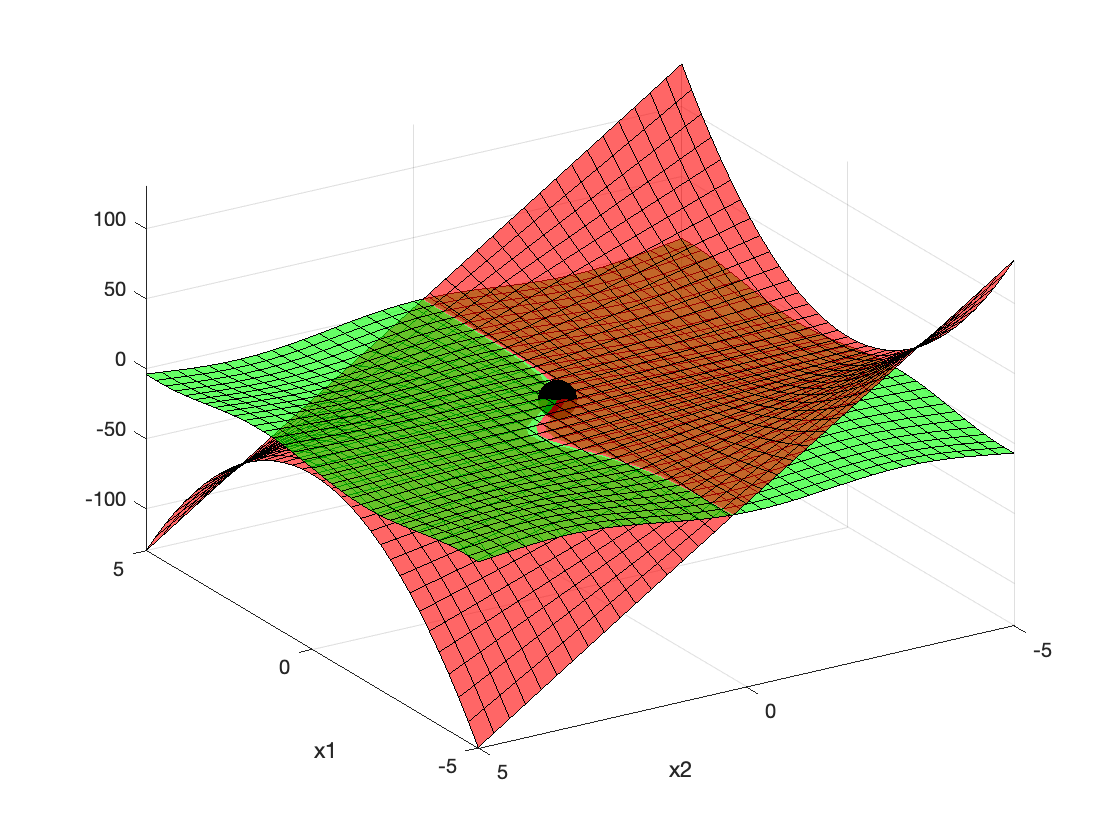
\includegraphics[width=8cm]{/Users/guilhermesalome/Teaching/Duke/Econ890 Matlab - 2019/supporting/matlab_system_nonlinear_equations.png}
\caption{\label{fig:orgc1a8959}
Solution of System of Nonlinear Equations.}
\end{figure}

We can display the progression of \texttt{fsolve} by specifying the \texttt{Display} option with the function \texttt{optimoptions}:
\lstset{language=matlab,label= ,caption= ,captionpos=b,firstnumber=1,numbers=left,style=Matlab-editor}
\begin{lstlisting}
options = optimoptions('fsolve', 'Display', 'iter');
x0 = [5; -5];
[x_root, fval_root] = fsolve(@system2d, x0, options);
\end{lstlisting}

It is possible to use \texttt{fsolve} with functions where the input is a matrix.
For example, to find the square-root of a matrix \(A\), we could create the following system:
\begin{align*}
f(X)=X*X - A
\end{align*}

We need to write the function above in a file:
\lstset{language=matlab,label= ,caption= ,captionpos=b,firstnumber=1,numbers=left,style=Matlab-editor}
\begin{lstlisting}
% sqrtA.m
function X = sqrtA(X0, A)
X = X0*X0 - A;
% function must return a vector
X = X(:);
\end{lstlisting}

We can now use \texttt{fsolve} to find the square-root of a matrix \(A\):
\lstset{language=matlab,label= ,caption= ,captionpos=b,firstnumber=1,numbers=left,style=Matlab-editor}
\begin{lstlisting}
% find the sqrt of A
A = eye(2);
X0 = rand(2);
X = fsolve(@(X) (sqrtA(X, A)), X0)
\end{lstlisting}
Observe that if a system has multiple solutions, \texttt{fsolve} will only find one.

\section{Finding the Root of a Nonlinear Function}
\label{sec:orge0a3896}
The function \href{https://www.mathworks.com/help/matlab/ref/fzero.html?s\_tid=doc\_ta}{\texttt{fzero}} can be used to find the root of a single nonlinear function.
That is, find the value \(x\) such that the nonlinear function \(f\) satisfies \(f(x)=0\).
Like \texttt{fsolve}, \texttt{fzero} will only find one root.
The function \texttt{fzero} uses a method similar to the bisection method, which requires the function \(f\) to have a change in sign.
If \(f\) does not change sign, then \texttt{fsolve} will not be able to find its root.
For example, \texttt{fsolve} cannot find the root of \(f(x)=x^2\).

The initial guess taken by \texttt{fzero} can be a scalar or a vector with two values.
If it is a scalar, say \(x_0\), then \texttt{fzero} tries to find another point \(x_1\) with the opposite sign of \(f(x_0)\), and then applies the bisection method to shrink the interval until a solution is reached.
If it is a vector, say \(\begin{bmatrix}x_0 & x_1\end{bmatrix}\), then \texttt{fzero} checks that \(f(x_0)\) and \(f(x_1)\) have different signs, and then applies the bisection method.
However, it shows an error if the signs are not different.

\lstset{language=matlab,label= ,caption= ,captionpos=b,firstnumber=1,numbers=left,style=Matlab-editor}
\begin{lstlisting}
% visualize polynomial
fun = @(x) x.^3 - 2*x.^2 + 3*x - 10;
fplot(fun)
% find root from initial guess (scalar)
x_min = fsolve(fun, -5);
hold on;
scatter(x_min, fun(x_min), 'ko', 'filled');
% find root from initial guess (vector)
x_min = fsolve(fun, [-5, 5]);
hold on;
scatter(x_min, fun(x_min), 'ro', 'filled');
\end{lstlisting}
\section{Assignment}
\label{sec:orga0aff60}
\begin{problem}
(Conditional Maximum Likelihood Estimator)
Consider the model:
\begin{align*}
Y = \beta_0 + \beta_1X + \varepsilon
\end{align*}
where \(\varepsilon\overset{d}{\sim}\Normal{\sigma^2}\).
We can write the conditional density of \(Y\vert X\) as the density of a normal (due to \(\varepsilon\)) with its mean shifted by \(\beta_0+\beta_1X\):
\begin{align*}
f_{\Set{Y\vert X}}(y)=\frac{1}{\sqrt{2\pi\sigma^2}}\e{-\frac{(y-(\beta_0+\beta_1X))^2}{2\sigma^2}}
\end{align*}
We can use this density to write the (conditional) likelihood given i.i.d. observations \(\Set{Z_i\equiv(Y_i, X_i)}_{i=1}^n\):
\begin{align*}
L(\beta_0,\beta_1,\sigma; Z) = \Pi_{i=1}^n f_{\Set{Y\vert X}}(y; \beta_0,\beta_1,\sigma)
\end{align*}
Thus, we can write the (conditional) maximum likelihood estimator for \(\beta_0\), \(\beta_1\) and \(\sigma\) as:
\begin{align*}
(\hat{\beta}_0, \hat{\beta}_1, \hat{\sigma}) = \argmax_{\beta_0, \beta_1, \sigma}{\sum_{i=1}^n-\frac{1}{2}\ln{2\pi\sigma^2}-\frac{1}{2\sigma^2}(y_i-\beta_0-\beta_1x_i)^2}
\end{align*}

Given appropriate values for \(\beta_0\) and \(\beta_1\), simulate \(1000\) observations for \(X\) from a normal distribution.
Graph the likelihood function (or log-likelihood) given the observations.
\end{problem}

\begin{problem}
(continuation of previous problem)
Using the simulated data from the previous exercise, estimate the parameters with the \texttt{linreg\_ols} function.
Now, estimate the parameters with MLE.
You can use \texttt{fminunc} or \texttt{fminsearch} to find the estimates.
Compare the results.
\end{problem}

\begin{problem}
(continuation of previous problem)
Compute the gradient of the log-likelihood function.
Use \texttt{fminunc} and the gradient of the log-likelihood function to estimate the parameters via MLE.
You can supply the option \texttt{CheckGradients} on a test-run to let Matlab check if the gradient you supplied is similar to the gradient computed numerically (good for checking if your code is correct).
\end{problem}

\begin{problem}
(continuation of previous problem)
We can also supply the Hessian to the \texttt{fminunc} function.
To do so, we add a third output (the Hessian matrix) to the file of the function we are minimizing.
Then, we set the option \texttt{HessianFcn} to \texttt{'objective'}.
Use \texttt{fminunc} with the gradient and the Hessian of the log-likelihood function to estimate the parameters via MLE.
\end{problem}

\begin{problem}
(Probit)
The Probit model (see Example 7.3 of \citet{H2000} is used to analyze data where the dependent variable is binary (\(Y\in\Set{0, 1}\)).
In this context, we can write the conditional probability of \(Y\) as:
\begin{align*}
  \begin{cases}
    \mathbb{P}(Y=1\vert X; \theta) &= \Phi(X'\theta)\\
    \mathbb{P}(Y=0\vert X; \theta) &= 1 - \Phi(X'\theta)
  \end{cases}
\end{align*}
where \(\Phi\) is the cdf of the standard normal distribution, \(X\) is a vector of independent random variables and \(\theta\) is a vector of unobserved parameters.
It is possible to write the conditional probability of \(Y\) in a single equation, since \(Y\) can only take binary values:
\begin{align*}
\mathbb{P}(Y\vert X;\theta)={\Phi(X'\theta)}^Y(1-\Phi(X'\theta))^{1-Y}
\end{align*}
Given i.i.d. observations \(\Set{(y_i, x_i)}_{i=1}^n\), we can write the (conditional) log-likelihood function for \(Z\equiv(Y,X)\) as:
\begin{align*}
l(\theta; Z)=\sum_{i=1}^n y_i\ln{\Phi(x_i'\theta)} + (1-y_i)\ln{1-\Phi(x_i'\theta)}
\end{align*}
Given appropriate values for \(\theta\), simulate \(1000\) observations for \(X\) from a normal distribution.
Graph the likelihood function (or log-likelihood) given the observations.
\end{problem}

\begin{problem}
(continuation of previous problem)
Estimate the parameters using MLE and \texttt{fminunc}.
\end{problem}

\begin{problem}
(Logit)
The Logit model (see page 508 of \citet{H2000}) is an alternative to the Probit model when it comes to analyzing binary data.
It can be argued that the interpretation of the parameters is more direct in the case of the Logit model.
We can write the conditional probability of \(Y\) as:
\begin{align*}
  \begin{cases}
    \mathbb{P}(Y=1\vert X; \theta) &= \Lambda(X'\theta)\\
    \mathbb{P}(Y=0\vert X; \theta) &= 1 - \Lambda(X'\theta)
  \end{cases}
\end{align*}
where \(\Lambda(v)=\frac{\e{v}}{1+\e{v}}\) is the cdf of the logistic distribution,\(X\) is a vector of independent random variables and \(\theta\) is a vector of unobserved parameters.
The above is equivalent to:
\begin{align*}
\mathbb{P}(Y\vert X;\theta)={\Lambda(X'\theta)}^Y(1-\Lambda(X'\theta))^{1-Y}
\end{align*}
Given i.i.d. observations \(\Set{(y_i, x_i)}_{i=1}^n\), we can write the (conditional) log-likelihood function for \(Z\equiv(Y,X)\) as:
\begin{align*}
l(\theta; Z)=\sum_{i=1}^n y_i\ln{\Lambda(x_i'\theta)} + (1-y_i)\ln{1-\Lambda(x_i'\theta)}
\end{align*}
Given appropriate values for \(\theta\), simulate \(1000\) observations for \(X\) from a normal distribution.
Graph the likelihood function (or log-likelihood) given the observations.
\end{problem}

\begin{problem}
(continuation of previous problem)
Estimate the parameters using MLE and \texttt{fminunc}.
\end{problem}

\begin{problem}
(continuation of previous problem) (Optional)
Derive the gradient and hessian of the log-likelihood in this case. (Hint: Equation (8.1.6) in \citet{H2000})
Estimate the parameters using MLE and \texttt{fminunc}, while supplying the gradient and hessian.
\end{problem}

\begin{problem}
(Dependent Observations)
Consider a Gaussian AR(1) process (see page 546 of \citet{H2000}):
\begin{align*}
y_t = \alpha + \beta y_{t-1} + \varepsilon_t
\end{align*}
where the \(\varepsilon_t\overset{d}{\sim}\Normal{\sigma^2}\) and are i.i.d, and \(\abs{\beta}<1\).
Simulate \(1000\) observations given an appropriate initial value for \(y_0\).

The log-likelihood in this case is given by:
\begin{align*}
  l(\theta; Z)=\frac{1}{n}\sum_{t=1}^n&\left[-\frac{1}{2}\ln{2\pi}-\frac{1}{2}\ln{\sigma^2}-\frac{1}{2\sigma^2}(y_t-\alpha-\beta y_{t-1})^2\right] +\\
& +\frac{1}{n}\left[-\frac{1}{2}\ln{2\pi}-\frac{1}{2}\ln{\frac{\sigma^2}{1-\beta^2}}-\frac{(y_0-\frac{\alpha}{1-\beta})^2}{2\frac{\sigma^2}{1-\beta^2}}\right]
\end{align*}
Implement the log-likelihood and estimate the parameters via MLE.
\end{problem}

\begin{problem}
(Model Selection)
We now consider the estimation of a linear regression via ordinary least-squares with the addition of a penalization term.
The penalization term is a function of the magnitude of the parameters of the model.
When we minimize the squared errors taking into account the penalization, some of the parameter estimates can be zero, leading to the estimation of a simpler model.
For a good overview, read this page on \href{https://en.wikipedia.org/wiki/Lasso\_(statistics)}{Lasso}.

Consider the model:
\begin{align*}
Y = \beta_0 + \sum_{i=20}\beta_i X_i + \varepsilon
\end{align*}
where \(\varepsilon\overset{d}{\sim}\Normal{\sigma^2}\), and each of the \(X_i\)'s are drawn from a normal distribution.

Fix the values of the \(\beta_i\)'s, but let \(\beta_1=\beta_2=0\).
Simulate the data for \(\Set{(Y_i, X_{i, 1}, \ldots, X_{i, 20})}_{i=1}^n\), with \(n=1000\).
Estimate the parameters via least-squares with \texttt{linreg\_ols}.
\end{problem}

\begin{problem}
(continuation of previous problem)
Estimate the parameters by minimizing the squared errors with the penalization term added:
\begin{align*}
&\min_{\beta_0,\beta_1,\ldots,\beta_{20}}{\frac{1}{n}\sum_{i=1}^n(y_i-\beta_0-\beta_1x_{i, 1} - \ldots - \beta_{20}x_{i, 20})^2}\\
&\text{subject to}\sum_{i=0}^{20}\abs{\beta}_i \leq \lambda
\end{align*}
for some \(\lambda > 0\).
Use the simulated data and the function \texttt{fmincon} in the estimation.
\end{problem}

\begin{problem}
(continuation of previous problem)
What happens to the parameters when \(n\) increases from \(1000\) to \(10,000\) and to \(100,000\)?
\end{problem}

\begin{problem}
(continuation of previous problem)
What happens to the final squared-errors of the regression when \(\lambda\) increases?
\end{problem}

\begin{problem}
(continuation of previous problem) (Optional)
Consider the Lagrangian form of the problem:
\begin{align*}
\min_{\beta_0,\beta_1,\ldots,\beta_{20}}{\frac{1}{n}\sum_{i=1}^n(y_i-\beta_0-\beta_1x_{i, 1} - \ldots - \beta_{20}x_{i, 20})^2 + \lambda\sum_{i=0}^{20}\abs{\beta_i}}
\end{align*}
The constrained problem was written as an unconstrained problem, and the parameters can now be estimated with \texttt{fminunc}.
Estimate the parameters and repeat the analysis from the previous two problems.
\end{problem}
\newpage
\printbibliography
\newpage
\end{document}